\section{A Case Study: VLIW Hardware/Software Design Space}
\label{sec:ee}
\subsection{Motivation}
In order to evaluate the behavior of the proposed approach
we will be using a parameterized Very Long Instruction
Word (VLIW) architecture~\cite{kathail_tr00} as testbed. The same philosophy
behind a VLIW system makes this a natural choice for several reasons:
\begin{itemize}
\item{Multi-Objective trade-offs}: VLIW architectures let designers
easily trade between power, energy and performances~\cite{}, resulting
in Pareto sets whose extension is an ideal ground for our testing
purposes focused on parameter-space space representation of Paretos.
\item{Compiler awareness}: Instruction Level Parallelism (ILP)
constitutes the key feature to enable the multi-objective trade offs
of the point above. It is statically obtained by the compiler which
performs code trasformations being aware of the underlying hardware
configuration.  This tight hardware/software dependence, makes the
VLIW scenario well suitable for investigating hardly predictable
hardware/software interactions, especially when compared to
architectures that, in order to preserve binary compatibility,
separate software generation processes from the hardware that
will execute it.
\end{itemize}

\subsection{Parameter Space}
System parameters can be classified in three main categories:
\emph{processor}, \emph{memory sub-system} and \emph{compiler}. 
The first is directly related to the VLIW core and includes the size
of the register files and the number of functional
units for each type. In particular, five different types of register
files are supported:
GPR (32-bit registers for integers), FPR (64-bit registers for
floating point values) PR (1-bit registers used to store the Boolean
values of predicated instructions), BTR (64-bit registers containing
information about possible future branches) and CR (32-bit control
registers containing information about the internal state of the
processor). The functional units involved are: \emph{Integer units},
\emph{floating point units}, \emph{memory units} (associated with
load/store operations) and \emph{branch units} (associated with branch
operations). With respect to the memory sub-system, the parameters
include \emph{size}, \emph{associativity} and
\emph{block size} for each of the three caches: First-level data cache
(L1D), first-level instruction cache (L1I) and second-level unified
cache (L2U).

Next, a set of the most impacting code compilation parameters has been
selected and included in the configuration space:
\begin{itemize}
\item{tcc\_region}: Specifies the scope of action of the compiler and the type
of code transformation involved (basic block, super block and hyper
block) 
\item {max\_unroll\_allowed}: The number of unroll iterations allowed
\item{regroup\_only}: Avoids inlining 
\item{do\_classic\_opti}: A set of classical optimization, not VLIW related,
such as common expression removal 
\item{do\_prepass\_scalar\_scheduling}: Performs a schedule before
forming regions 
\item{do\_postpass\_scalar\_scheduling}: Performs a schedule after the region formation 
do\_modulo\_scheduling  Modular scheduling 
\item{memvr\_profiled}: Performs a memory-dependencies profiling 
\end{itemize}

As regards the class of benchmark being considered, a set applications representative of some common
frequently running code kernels in an embedded multimedia
environment has been chosen. Table~\ref{tab:bench} shows the set of applications
along with a brief description.
\begin{table}
	\centering
	\caption{Benchmarks}
	\label{tab:bench}
	\begin{tabular}{ll}
	\hline
	\multicolumn{1}{c}{Benchmark} & \multicolumn{1}{c}{Application} \\
	\hline
	Alloca\_test & Memory array allocation test \\
	Bmm & Matrices multiplication and elements sum \\
	Fir\_int & Finite impulse response \\
	Mm & Floating point matrices multiplication \\
	Sha256 & Cryptocurrency header Hashing \\
	Wave & Wavefront computation \\
	\hline
	\end{tabular}
\end{table}

\subsection{Evaluation Metrics}

The results presented in the next section compare PS against one
widely adopted Multi-objective Genetic
Algorithm~\cite{knowles_techrep06}. At best of our knowledge, genetic
approaches in general still represent the best compromise between
efficiency (i.e. time required for exploration) and accuracy of the
reported Paret Sets.  Note that for the reasons described above,
mono-objective approaches have been explicitly excluded from this
analysis. Same decision has been taken for other approaches (e.g.
dependecy based~\cite{givargis_tvlsi02}) that make use of some
a-priori knowledge about the role and meaning of each parameter, since
our aim is evaluate the capacity of focusing on interesting parameter
regions without any external judgement or help based on euristics.
Finally, it should be pointed out that in this introductory work we
will explicitly use the SPEA~\cite{zitzler_eurogen01} variant of MOGA,
remainding to works like~\cite{zitzler_ec00}~\cite{zitzler_tec03} for
a detailed analysis on how it differs and what could be expected from
similar multi-objective strategies.

%------------------------------------------------------------------------------

\subsection{Results}

Set of Figures~\ref{fig:pareto_fronts_100}
and~\ref{fig:pareto_fronts_500} show the resultig pareto fronts for two
different scenarios of 100 and 500 simulations budget.

\begin{table*}
  \centering
  \begin{tabular}{ccc}
    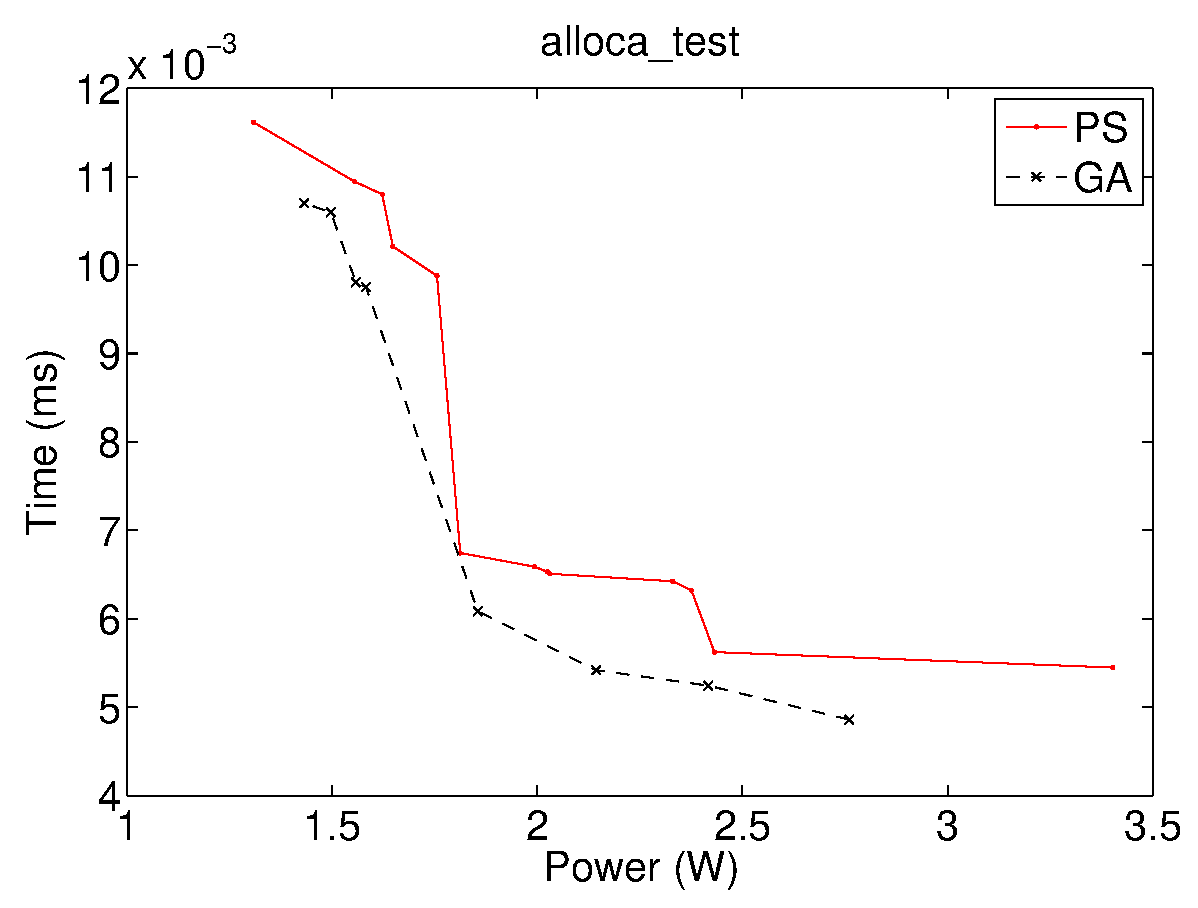
\includegraphics[width=0.30\textwidth]{pictures/alloca_100.eps} &
    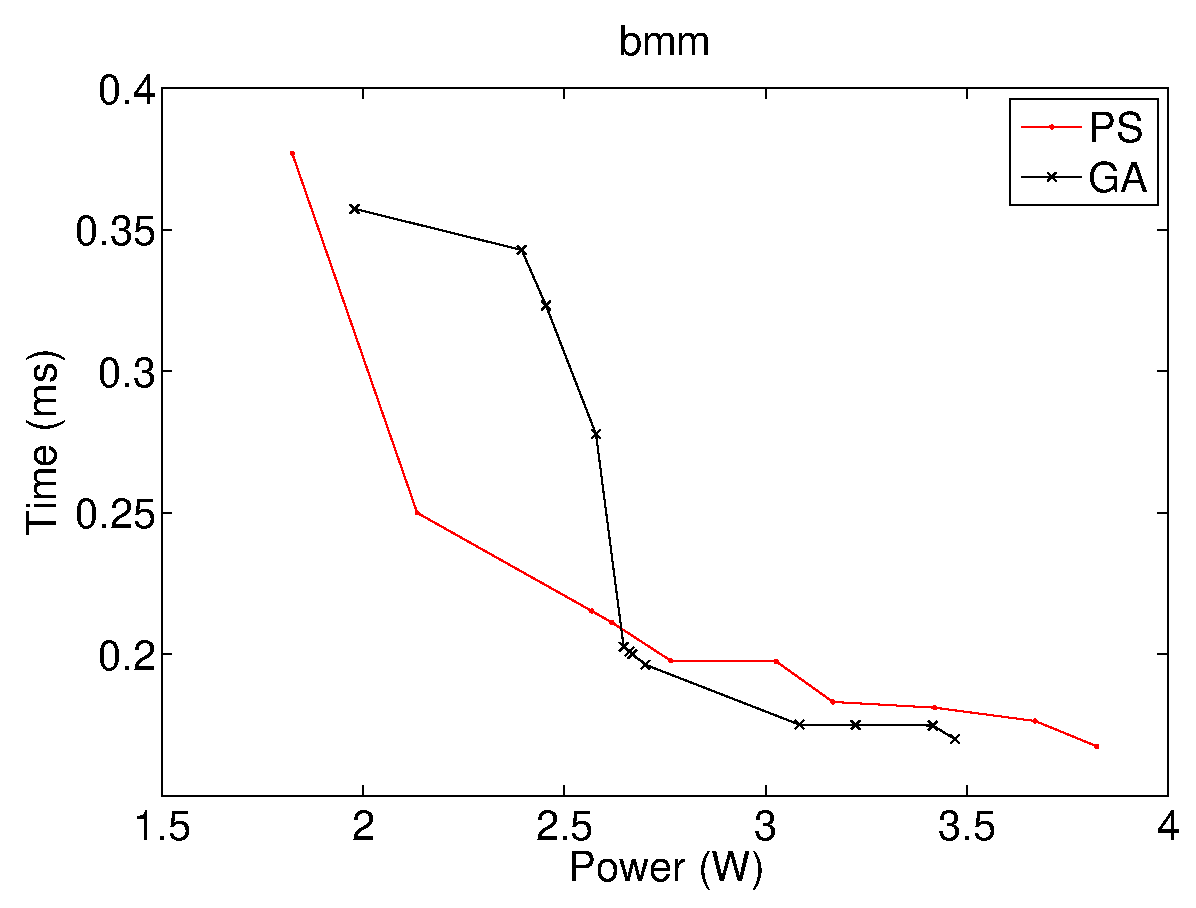
\includegraphics[width=0.30\textwidth]{pictures/bmm_100.eps} & 
    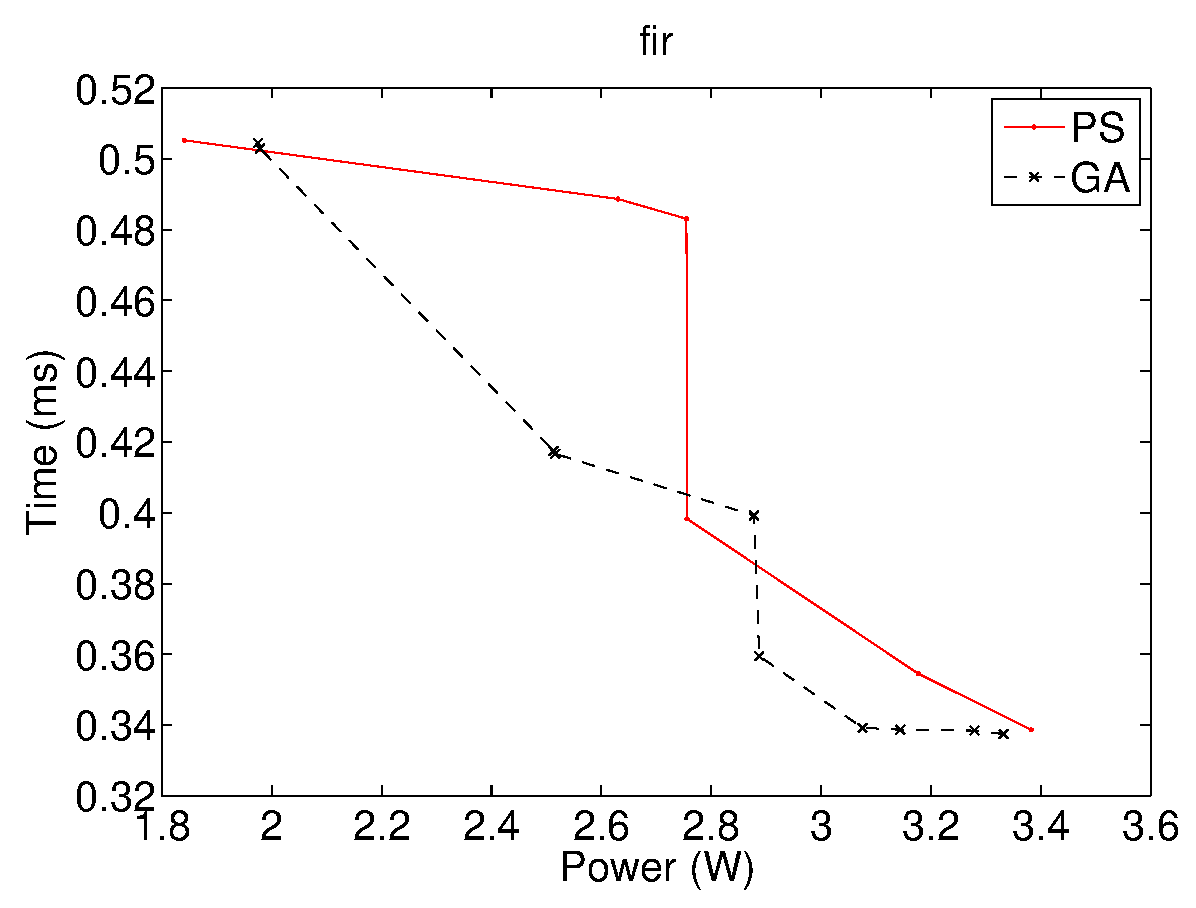
\includegraphics[width=0.30\textwidth]{pictures/fir_int100.eps} \\
    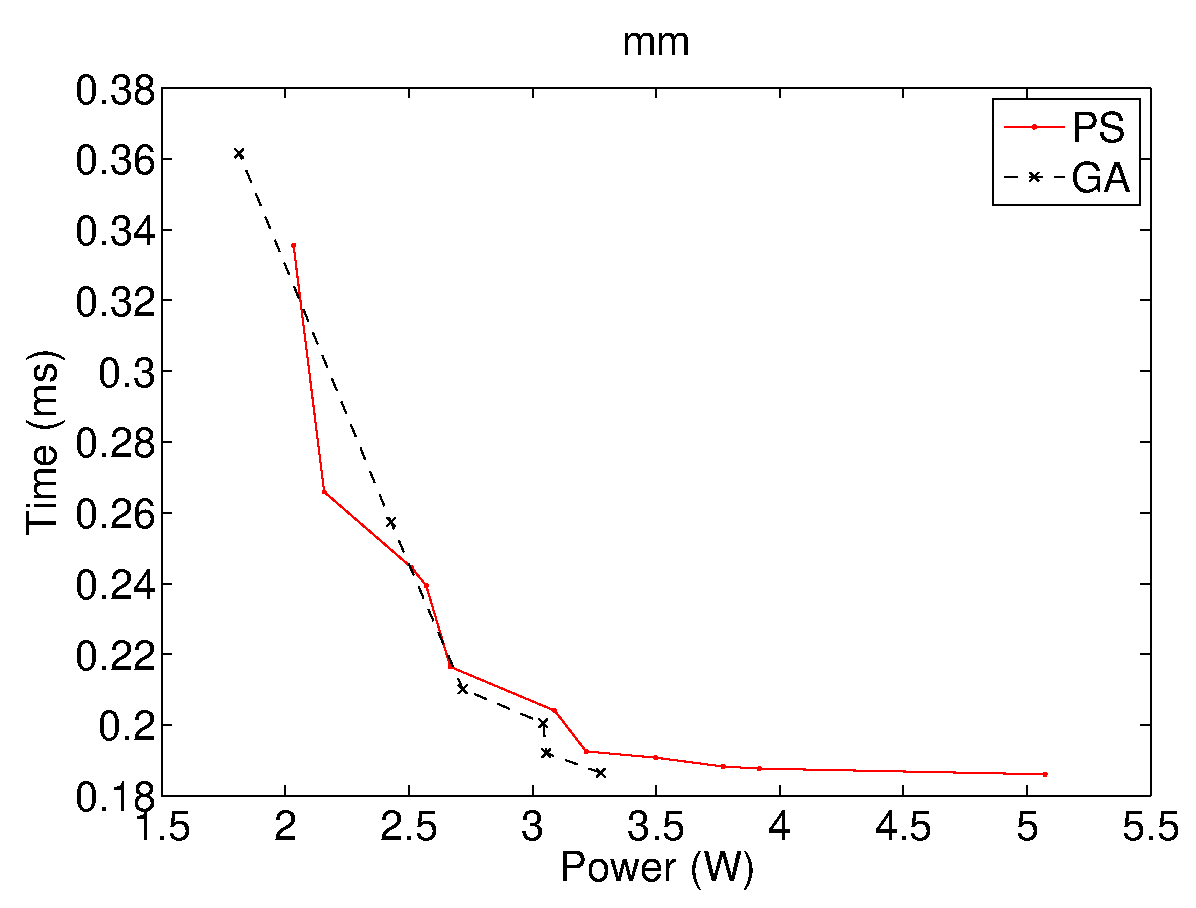
\includegraphics[width=0.30\textwidth]{pictures/mm_100.eps} &
    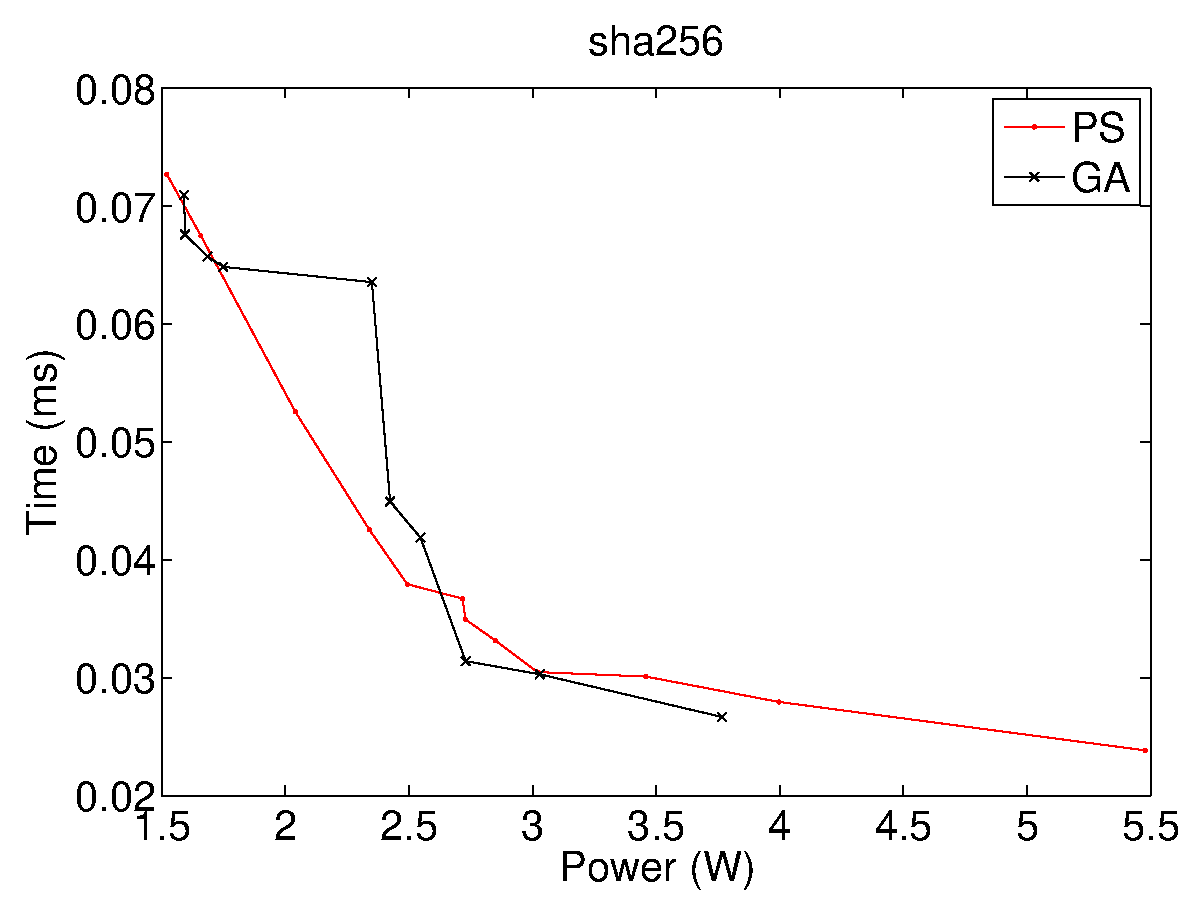
\includegraphics[width=0.30\textwidth]{pictures/sha_100.eps} &
    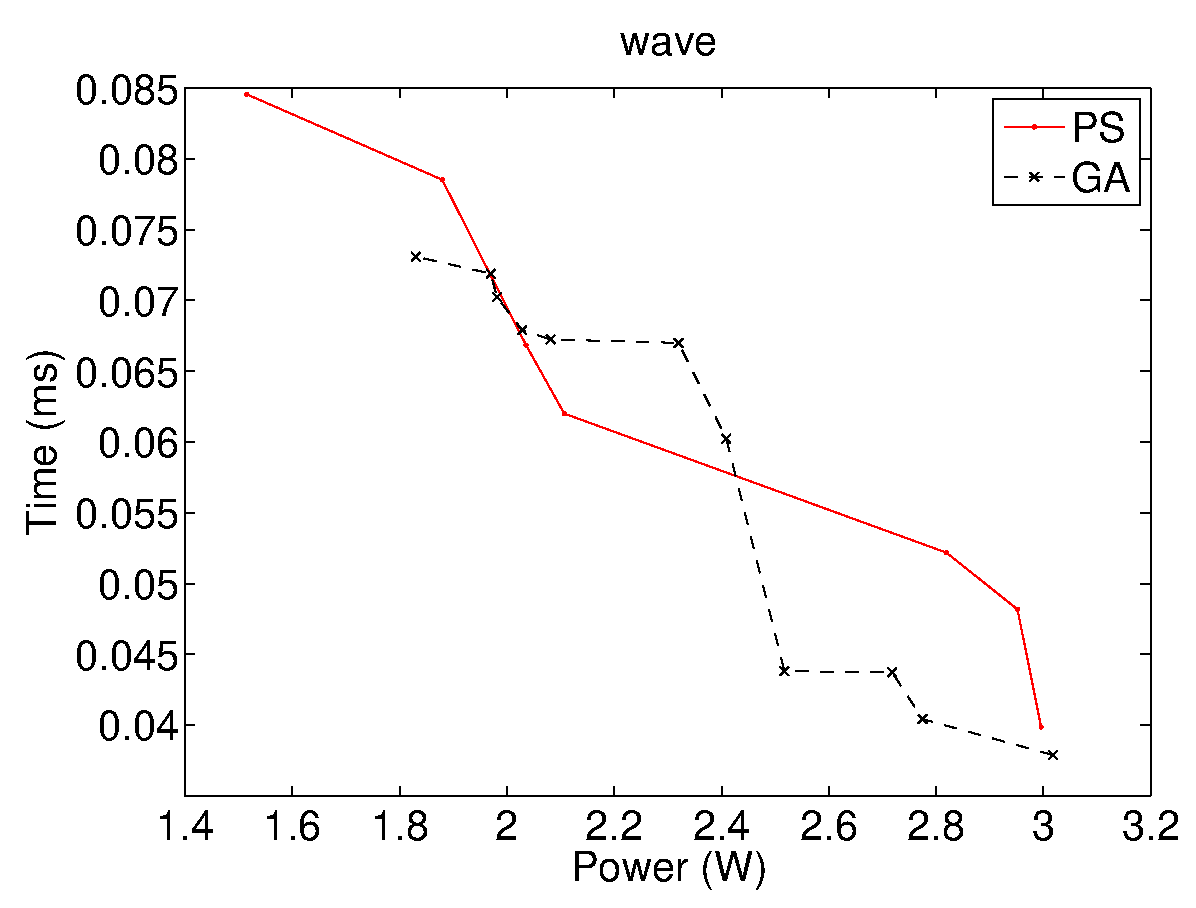
\includegraphics[width=0.30\textwidth]{pictures/wave_100.eps} 
  \end{tabular}
  \caption{Pareto fronts found by PS and GA for a fixed budget of 100 configurations.}
  \label{fig:pareto_fronts_100}
\end{table*}

\begin{table*}
  \centering
  \begin{tabular}{ccc}
    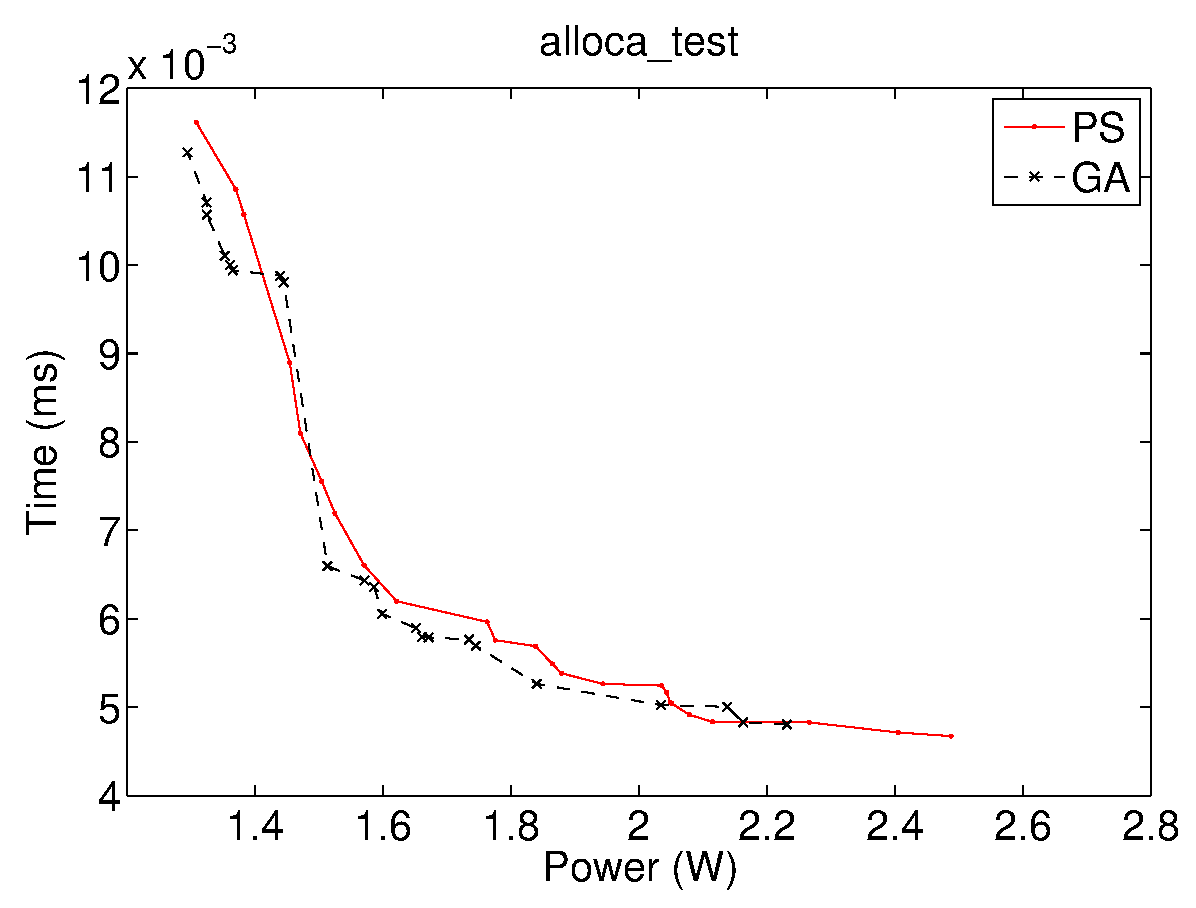
\includegraphics[width=0.30\textwidth]{pictures/alloca_500.eps} &
    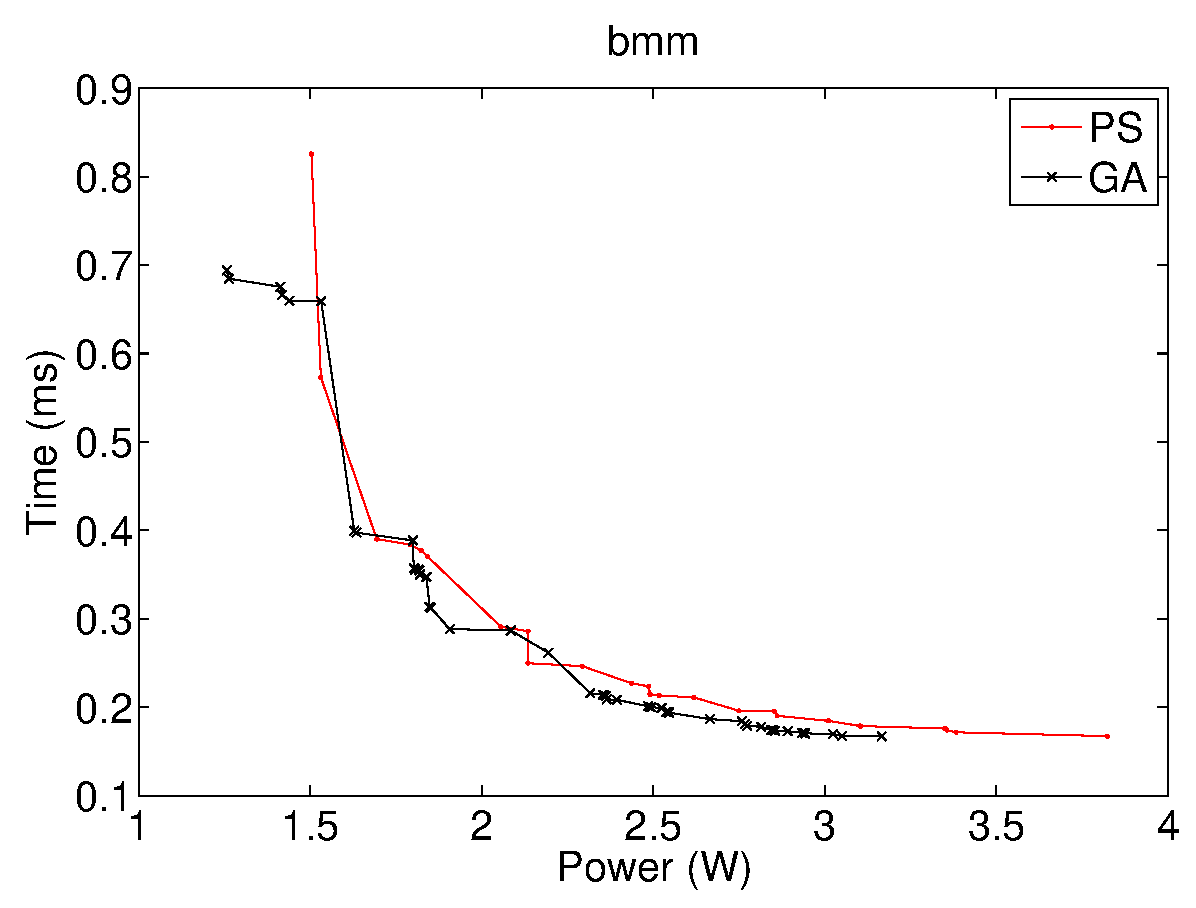
\includegraphics[width=0.30\textwidth]{pictures/bmm_500.eps} & 
    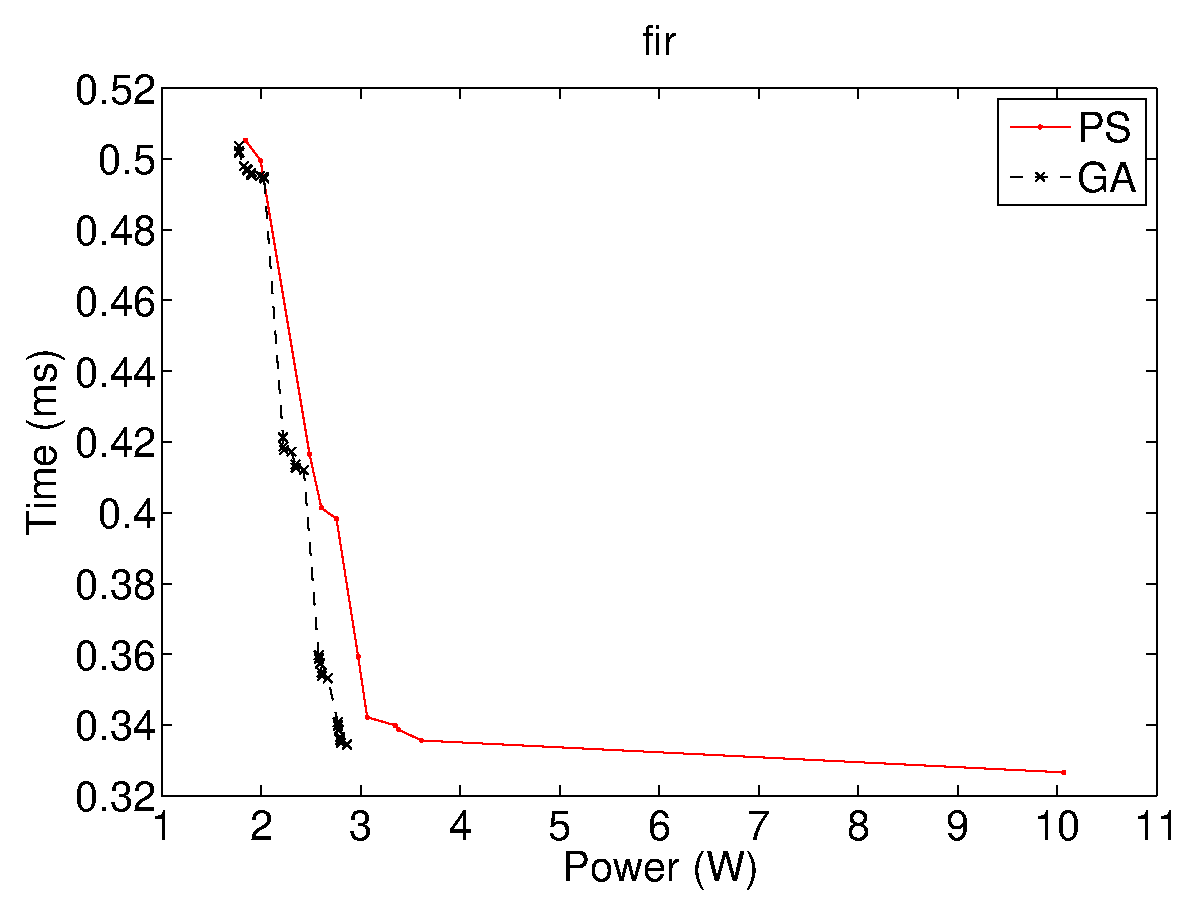
\includegraphics[width=0.30\textwidth]{pictures/fir_int500.eps} \\
    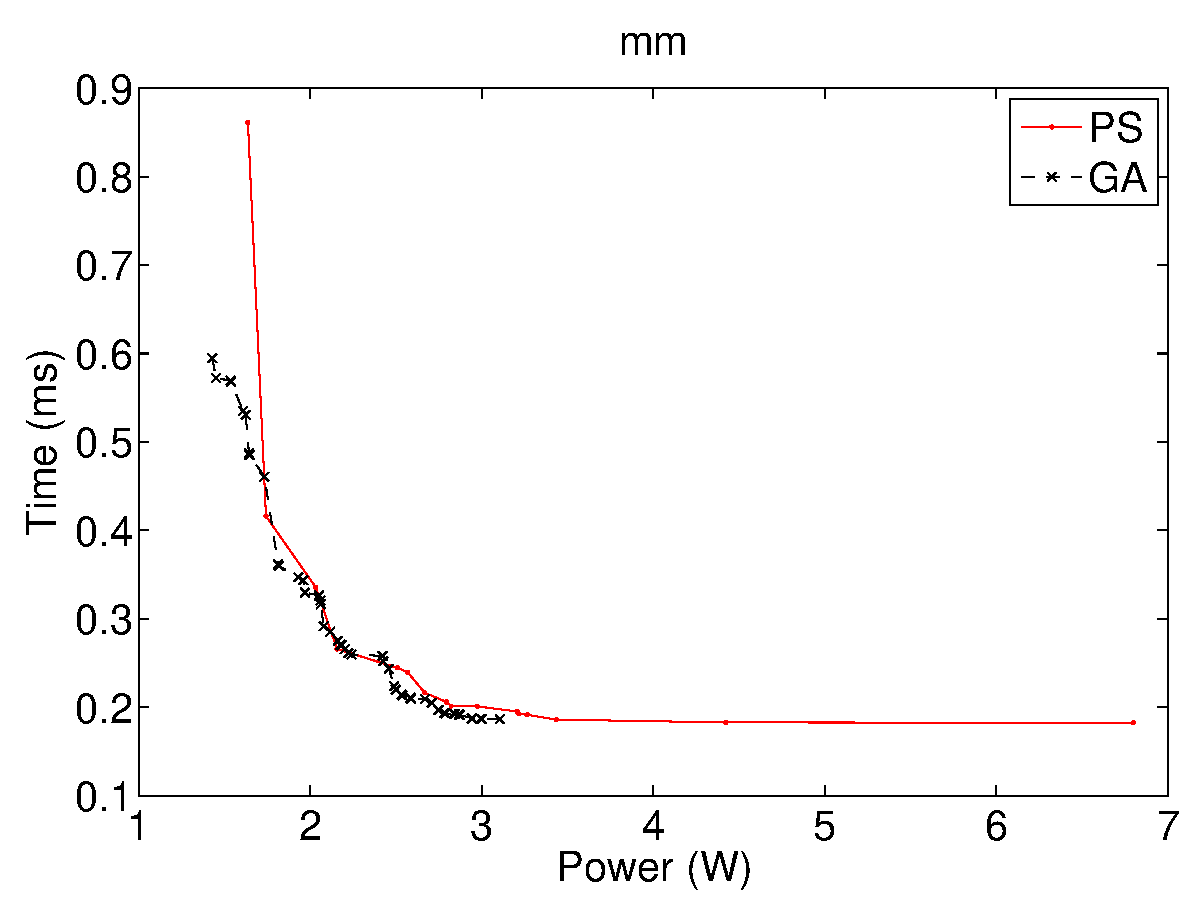
\includegraphics[width=0.30\textwidth]{pictures/mm_500.eps} &
    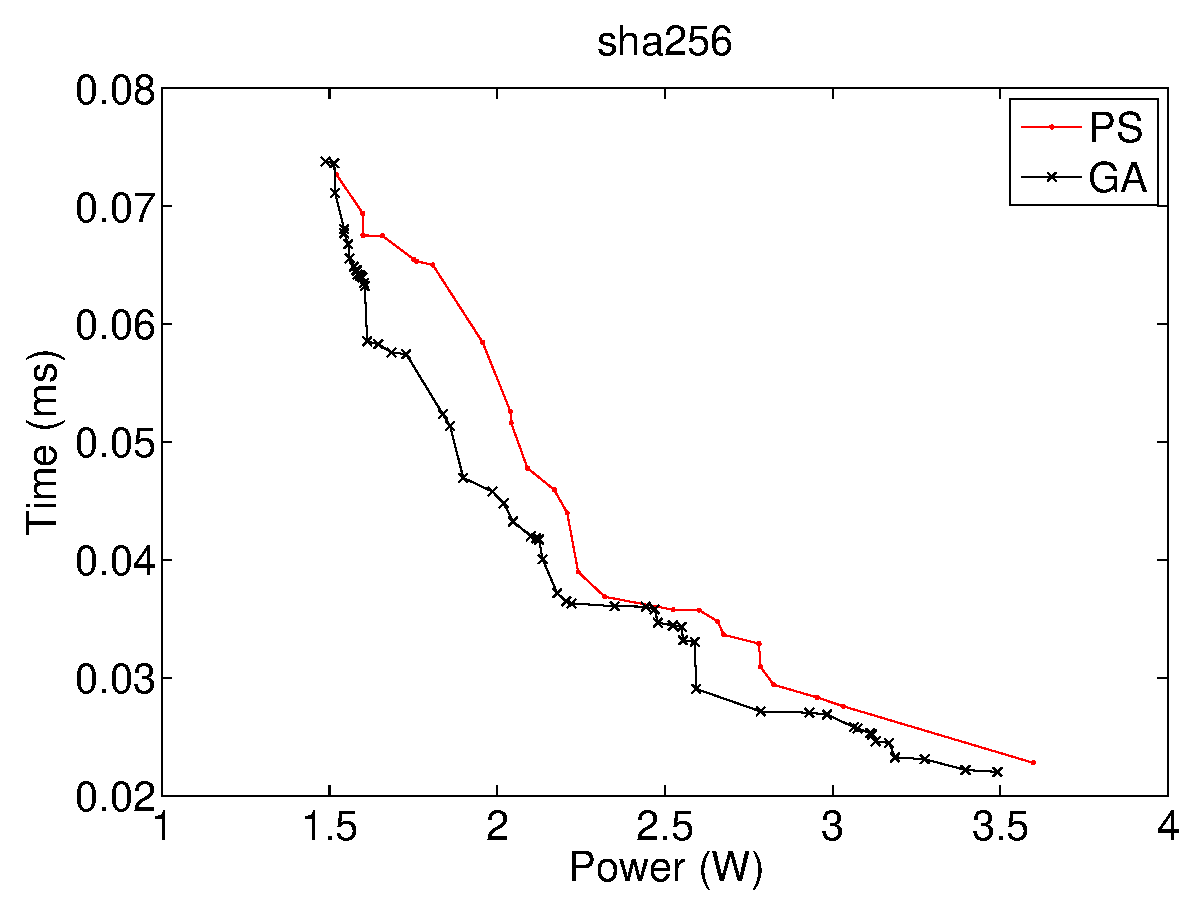
\includegraphics[width=0.30\textwidth]{pictures/sha_500.eps} &
    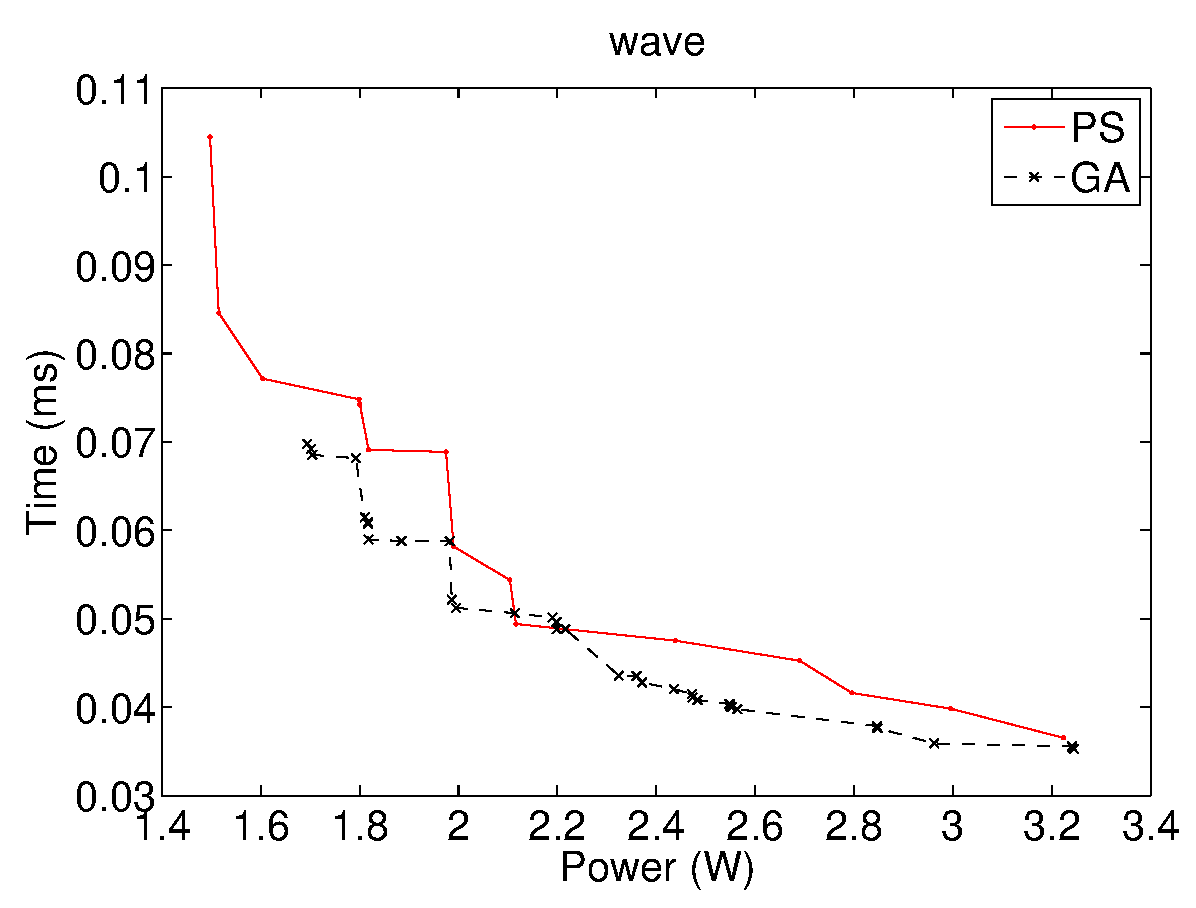
\includegraphics[width=0.30\textwidth]{pictures/wave_500.eps} 
  \end{tabular}
  \caption{Pareto fronts found by PS and GA for a fixed budget of 500 configurations.}
  \label{fig:pareto_fronts_500}
\end{table*}

As can be seen TODO...


In order to evaluate the Paretos from a quantitative point-of-view we
will consider two metrics, namely, the \emph{variation range} and the
\emph{average normalised absolute dispersion error}. For a given
objective, the variation range represents the ratio between the
maximum and the minimum value observed for that objective. A
comparison between the variation range for different benchmarks
between a FCP and a VCP exploration for both power dissipation and
execution time is shown in Fig.~\ref{fig:dispersion}(a) and (b)
respectively. As it can
be observed, the VCP exploration provides solutions which fall on a
range that is, on average, 23\% and 40\% wider than that provided by a
FCP exploration for power dissipation and execution time,
respectively.
\begin{table}
  \centering
  \begin{tabular}{c}
    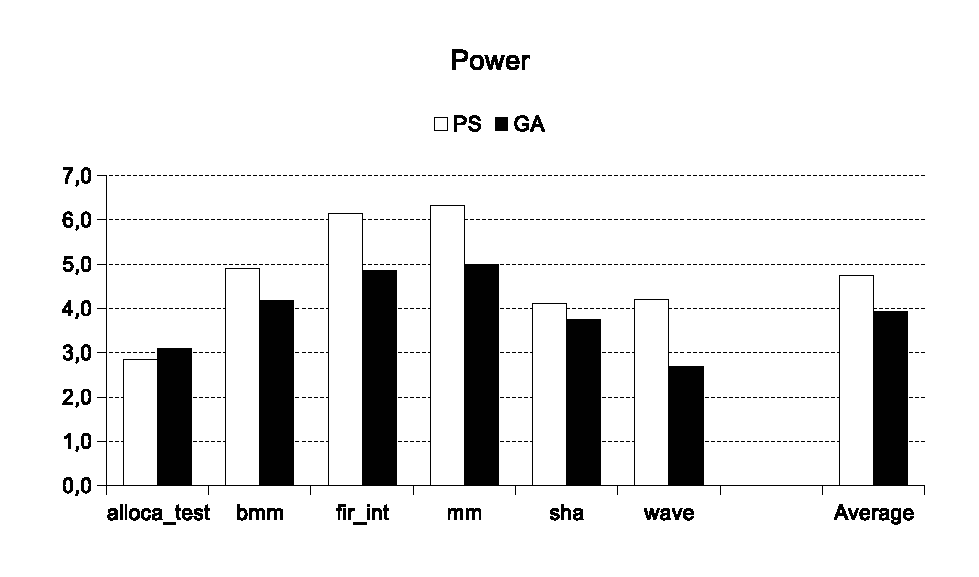
\includegraphics[width=0.4\textwidth]{pictures/variation_power.eps} \\
    (a) \\
    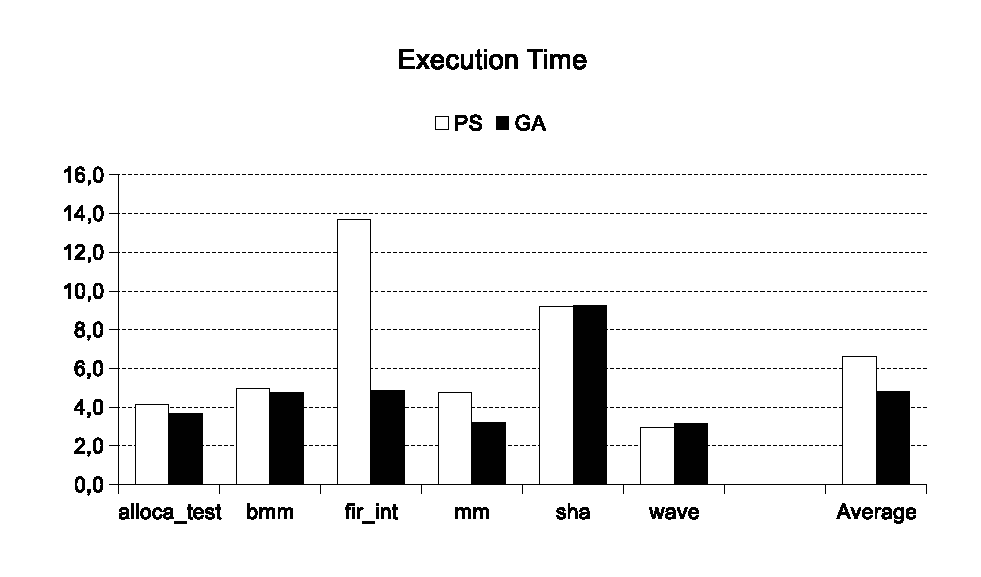
\includegraphics[width=0.4\textwidth]{pictures/variation_etime.eps}
    (b) \\
    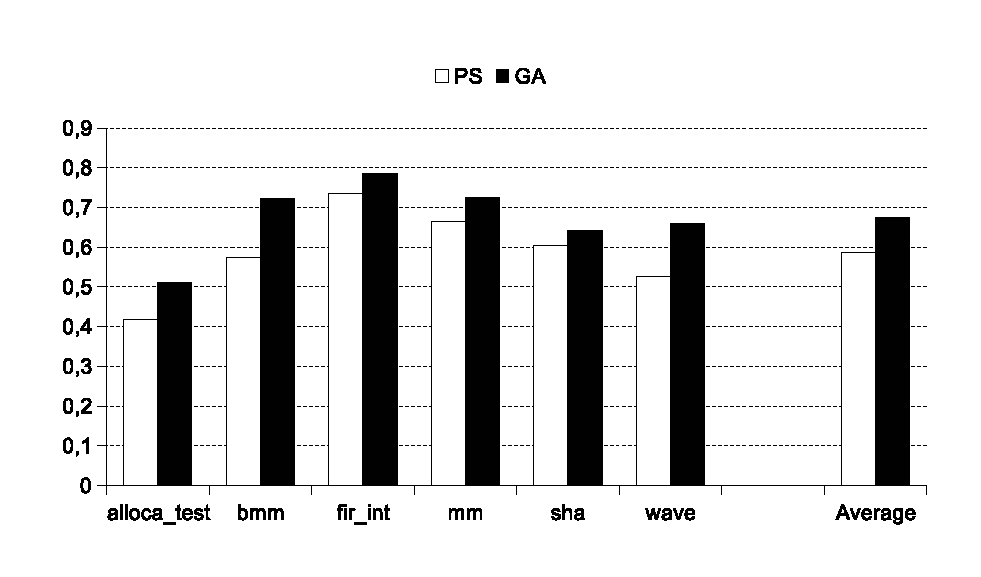
\includegraphics[width=0.4\textwidth]{pictures/dispersion.eps} \\
    (c) 
  \end{tabular}
  \caption{(a)(b) Variation range for different benchmarks between PS and GA
  and average dispersion absolute dispersion (c)}
  \label{fig:dispersion}
\end{table}


The average normalised absolute dispersion error measures
the average absolute difference between the distribution of points in
the objective space and an ideal distribution in which the points are
uniformly distributed over the objective space. Formally, let $O$ be
the image, in the objective space, of the configurations visited by
the design space exploration. The generic element of $O$ (\ie, a
solution) is a pair $(p,t)$ where $p$ and $t$ are the average power
and execution time, respectively. The two-dimensional objective space
is then partitioned by a $M_x \times M_y$ mesh. For each tile $T_i,
\ i=1, 2, \ldots, M_xM_y$ of the mesh, let $N_i$ be the number
of points in $O$ which fall in $T_i$. The average absolute error, $E_i$, for
$T_i$ is the absolute value of the difference between $N_i$ and the
ideal number of solutions, $\overline{N}$, which should fall in $T_i$
in case of uniform distribution. Such $\overline{N}$ can be simply
computed as the ratio between the cardinality of $O$ and the number of
tiles. Thus,
\[ E_i = |N_i - \overline{N}|, \]
where $\overline{N} = |O| / (M_x M_y)$. The average
normalised absolute dispersion error ($ANADE$) is the average of $E_i$
normalised to the maximum absolute error $E_{max}$:
\[ ANADE = \frac{\sum_{i=1}^{M_xM_y} E_i/(M_xM_y)}{E_{max}}, \]
where $E_{max}$ can be computed as the average absolute error in the worst
case in which all the solutions fall in a single tile:
\[ E_{max} = \frac{(M_x M_y - 1) \overline{N} + |\overline{N} -
    |O|| }{M_x M_y}. \] 

Fig.~\ref{fig:dispersion}(c) shows the average normalised absolute
dispersion errors for different benchmarks for FCP and VCP
exploration. As it can be observed, VCP exploration reduces the
dispersion error on average by 20\% as compared to a FCP exporation.
